\chapter{Data preprocessing}

The available data volumes have to be preprocessed before being used in the neural network classifier.
The preprocessing steps consist of re-sampling, slicing, contrast enhancement and cropping.  

There is not one obvious way to combine the different datasets and available labels in one project.
The chosen approach in this work is discussed below.
First, the convertion of the full class labels to point labels is discussed. 
Secondly, the split of the datafiles in a train set, a validation set and a test set is discussed.

\section{Image preprocessing}

A (medical) image\footnote{In this work, I use \textit{image} to refer both to 2-dimensional and 3-dimensional images.} consists of a combination of data - the pixel
\footnote{A \textit{pixel} (picture-element) is the smallest component of a digital bitmap image. 
It is defined by a position vector and carries $c$ values. Where $c$ is the number of channels of the image. 
Sometimes, a pixel of a 3-dimensional digital image is called a \textit{voxel} (volume element).} 
values - and metadata.

For a medical image, there are two types of metadata:
\begin{description}
    \item [Describing the patient \& medical data:] patient identification, pathologies, date of scan, date of birth, gender, weight, height,\dots
    \item [Technical meta-data:] The size (number of pixels per dimension), pixel spacing (distance between pixels along a dimension), orientation vector, image modality \& other information regarding the image aquisition.
\end{description}

For a discussion of the data used in this work, chapter \ref{sec:datasets} can be consulted. 

\subsection{Resampling and slicing\label{sec:resampling}}

In figure \ref{fig:AllDataset_dims}, the differences regarding the dimension and resolution for the different volumes in the combined dataset are illustrated. 
It is necessarily to uniformize the data input to the network. 
This requires uniformization of the image spacing vector in all directions\footnote{A typical \acrshort{cnn} is not scale-invariant.}. 
I chose to resample on a $1mm\times 1mm \times 1mm$ isotropic grid. 
If necessary, images are rotated to uniformize the orientation vectors. 
Every image is now a 3-dimensional array\footnote{Both \acrshort{ct} and \acrshort{mri} images have only 1 channel.} with the same sequency of dimensions and the same spacing along these dimensions.
The chosen uniform dimension sequence is:
\begin{enumerate} 
    \item Craniocaudal axis; perpendicular to the transverse plane.
    \item Anteroposterior axis; perpendicular to the coronal (frontal) plane.
    \item Left-right axis; perpendicular to the sagittal plane.
\end{enumerate}
The inputs for the 2D models are obtained by \textit{slicing} the volume along one of the dimensions.
This means that from each scan volume, three different sets of two-dimensional slices can be generated, depending on the slicing axis\footnote{The slicing axis is the axis perpendicular to which ones slices the volume}.

When resampling the image itself, linear interpolation is used. 
To resample the classification masks on a new grid, the \textit{nearest neighbor} method is used\footnote{
    SimpleITK \cite{sitk} provides useful tools to perform these operations.
    } 
since factorial data must not be interpolated. 

\subsection{Contrast enhancement}
To two-dimensional images obtainded from slicing the volumes are preprocessed with the \acrfull{clahe} algorithm. 
The difference with ordinary histogram equalization is that the \acrshort{clahe} method calculates different histograms for different sections of the image.
This technique allows to improve the local contrast in each region of an image.
When an image contains regions that are significantly lighter or darker than the rest of the image (as is the case for both \acrshort{ct} and \acrshort{mri} images) the AHE methods perform better than histogram equalization based on the complete image.

\begin{SCfigure}[][htb]
    \centering
    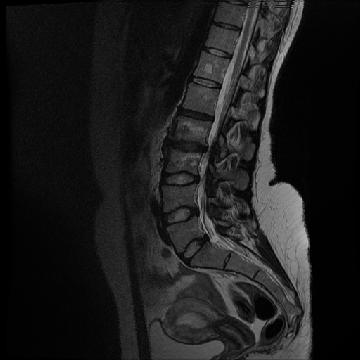
\includegraphics[width=.32\textwidth]{images/orig_usieg8_s22.jpg}
    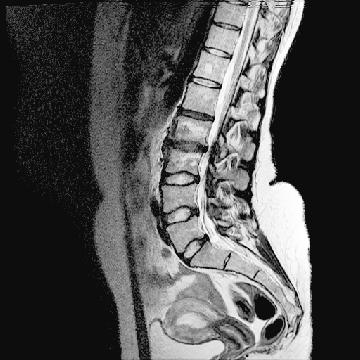
\includegraphics[width=.32\textwidth]{images/hist_usieg8_s22.jpg}
    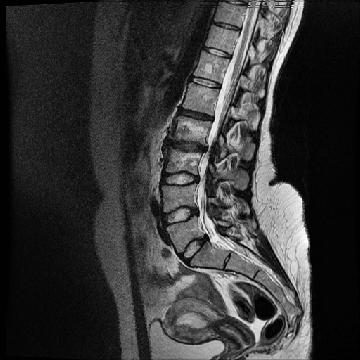
\includegraphics[width=.32\textwidth]{images/clahe_usieg8_s22.jpg}
    \caption{Image: 22$^{th}$ sagittal slice of the 8$^{th}$ image of the USiegen dataset. 
    From left to right, the original image, the image after ordinary histrogram contrast enhancement and the result after \acrshort{clahe}.
    The images show that \acrshort{clahe} avoids increasing the noise in the larger dark areas while resulting in a more balanced image than the ordinary histogram method.
    }
\end{SCfigure}

\acrfull{clahe} is an improvement on adaptive histogram equalization.
By limiting the contrast amplificiation, it avoids that noise is amplified in (near) constant regions of the image.
The parameters of this operation were adjusted manually.
Based on trail and error iterations, where the quality of the contrast improvement was estimated with the human eye based on visualizations from all datasets,
the following parameterset was chosen:
\begin{description}
    \item[Number of grey bins:] 256 (maximum possible when working with 8-bit encoded images).
    \item[Kernel size:] 50. This parameter defines the extend of the \textit{local} region used by the algorithm.
    \item[clip limit:] $9.10^{-3}$. This parameter suppresses noise in the most dark regions (which contain least information).
\end{description}

\section{Train, validation and test split considerations\label{sec:trainValTestSplit}}

To allow evaluation of the models produced, a test set is split from the development set.
The objective is to evaluate how well a model generalizes to new data\footnote{
    New data is to be interpreted here a new sample from \textit{the same population} as the development sample.
    Unfortunately, I cannot claim that the different datasets I collected certainly form a perfect representation of the population of medical images of the lumbar spine.}. 
To provide an honest estimate of the out-of-sample performance, the test dataset should be representative of the investigated population and (hidden) correlations with elements of the development sample should be avoided.

This is done\footnote{
    To accomplish this, I used the function \texttt{GroupedStratifiedSplit} at \url{https://github.com/scikit-learn/scikit-learn/pull/18649/}. 
    This class is not yet part of the official \texttt{sci-kit learn} library release (at the time of writing), but functions well for this application.} taking into account the following:
\begin{description}
    \item[Stratified data:] The combination of data from different sources is obviously stratified. Every source is considered a subpopulation. The datasplit is made such that the proportion of scans orginating from each datasource in every split is proportional to their occurance in the total population.
    \item[Grouped data:] The scans of the same patient can be assumed to be correlated to eachother. These scans should not be spread over different splits. The data is split at patient level.
\end{description}

\todo{Table with split}